\section{Results}
\label{sec:-res}
We find that our model of user accuracy is accurate within bounds

\begin{figure}[bht]
\centering
 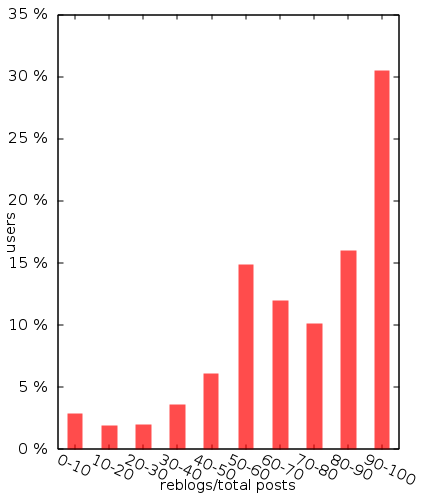
\includegraphics[width=3.5in]{degree}
  \caption{The bins on the X axis represent percentages of users, grouped by what percentage of their posts are reblogs.  The Y axis indicates the magnitude of the membership within this group.  Overall, we observe that blogs contain an average of 70\% reblogged material, and a median amount of 76\% reblogged material.}
  \label{fig:-deg}
\end{figure}

Figure \ref{fig:-deg} indicates that the majority of users spend more 
time reblogging others' content than adding their own to the network.


Figure \ref{fig:-pop} shows us that the most popular posts are text 
posts, followed most closely by image posts.  This suggests that Tumblr 
is not so far removed from classic blogging sites.
gifsets\cite{hillman2014tumblr}

\begin{figure}[bht]
\centering
 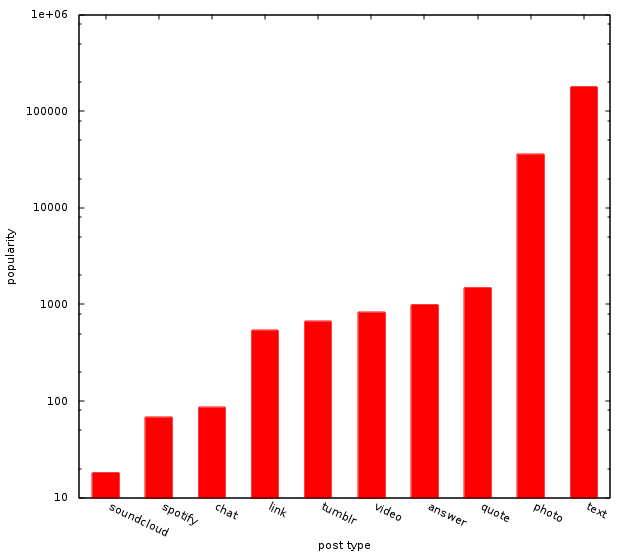
\includegraphics[width=3.5in]{popularity}
  \caption{The graph represents the relative popularity of all surveyed post types.  Note that the graph has a log scale on the y axis}
  \label{fig:-pop}
\end{figure}
This is particularly interesting in light of the 

%%% Local Variables: 
%%% mode: latex
%%% TeX-master: "main"
%%% End: 
